\documentclass{article}
\usepackage{graphicx} % Required for inserting images
\usepackage[italian]{babel}
\usepackage{amsmath}
\usepackage[hidelinks]{hyperref}
\usepackage[dvipsnames]{xcolor}
\usepackage{float}
\usepackage{algorithm}
\usepackage{algpseudocode}
\usepackage{multicol}

\newcommand{\df}[1]{\noindent\textbf{Definizione } #1.\newline}

\title{Sicurezza}
\author{Leonardo Ganzaroli}
\date{}

\begin{document}

\maketitle

\addcontentsline{toc}{section}{\protect\numberline{}Introduzione}

\tableofcontents

\newpage

\hypersetup{allcolors=black}

\section*{Introduzione}

Questi appunti del corso \textit{Sicurezza} sono stati creati durante la laurea Triennale di informatica all'università "La Sapienza".

\newpage

\section{Elementi introduttivi}

La sicurezza informatica si occupa delle risorse informatiche soggette a diversi tipi di minacce e le misure necessarie a garantirne la protezione.\newline

\noindent I 3 obiettivi chiave sono:
\begin{enumerate}
    \item \textbf{Confidenzialità}
        \begin{itemize}
            \item Dei dati
            \item Privacy
        \end{itemize}
    \item \textbf{Integrità}
        \begin{itemize}
            \item Dei dati
            \item Dei sistemi
        \end{itemize}
    \item \textbf{Disponibilità}\newline
\end{enumerate}

\noindent Altri 2 fattori importanti sono:
\begin{enumerate}
    \item \textbf{Autenticità}
    \item \textbf{Responsabilità}\newline
\end{enumerate}

\begin{figure}[ht]
    \centering
    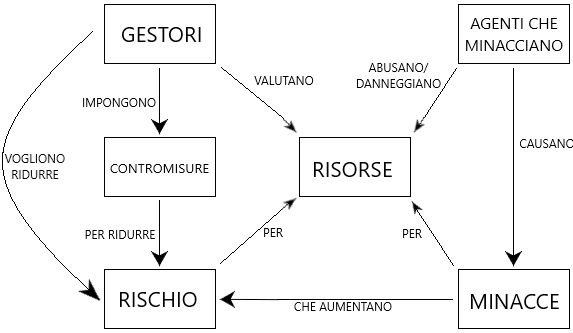
\includegraphics[width=0.8\linewidth]{SCHEMA.png}
    \caption{Modello generale}
\end{figure}

\df{(Agenti che minacciano) Avversario = individuo/gruppo/organizzazione che vuole condurre o conduce attività dannose}

\df{Attacco = qualsiasi tipo di attività malevola che tenta di raccogliere/negare/distruggere/$\ldots$ le risorse o i dati di un sistema informativo}

\df{Contromisura = tecnica o dispositivo che compromette l'efficacia di un'attivita indesiderata}

\df{Rischio = misura della portata di una minaccia su un'entità}

\df{Politica di sicurezza = insieme di criteri per la fornitura dei servizi di sicurezza}

\df{Minaccia = circostanza o evento con il potenziale di avere un impatto negativo}

\df{Vulnerabilità = Debolezza di un sistema informativo, delle sue procedure, dei suoi controlli interni o della sua implementazione che potrebbe essere sfruttata da una minaccia}

\df{Attacco = minaccia che viene eseguita ed eventualmente porta ad una violazione}

\noindent Le principali conseguenze degli attacchi (ed i rispettivi attacchi) sono:
\begin{itemize}
    \item Divulgazione non autorizzata
        \begin{itemize}
            \item Esposizione
            \item Intercettazione
            \item Inferenza
            \item Intrusione
        \end{itemize}
    \item Inganno
        \begin{itemize}
            \item Mascheramento
            \item Falsificazione
            \item Ripudio
        \end{itemize}
    \item Usurpazione
        \begin{itemize}
            \item Appropriazione indebita
            \item Uso improprio
        \end{itemize}
    \item Interruzione
        \begin{itemize}
            \item Interdizione
            \item Corruzione
            \item Ostruzione
        \end{itemize}
\end{itemize}

\noindent Gli attacchi si possono dividere in:
\begin{itemize}
    \item \textbf{Attivi} se cercando di influenzare il funzionamento del sistema
    \item \textbf{Passivi} se cercano di apprendere informazioni senza toccare le risorse\newline
\end{itemize}

\section{Autenticazione degli utenti}

\subsection{Modello}

\df{L'autenticazione digitale degli utenti è un processo atto a stabilire la fiducia nelle identità fornite dagli utenti ad un sistema informativo}

\noindent Il processo si divide in:
\begin{enumerate}
    \item \textbf{Identificazione}

        L'utente fornisce una presunta identità.
    
    \item \textbf{Autenticazione}

        Si stabilisce la validità dell'identità presentata.\newline
    
\end{enumerate}


\noindent Un modello per rappresentare il procedimento è l'SP800-63-3:

\begin{table}[ht]
    \centering
    \begin{tabular}{|c|}
        \hline
        \textbf{Requisiti base}\\
        \hline
        Identificazione\\
        \hline
        Autenticazione\\
        \hline
        \textbf{Requisiti derivati}\\
        \hline
        Uso autenticazione a più fattori\\
        \hline
        Usare meccanismi resistenti\\
        \hline
        Evitare riutilizzo identificatori per tot. tempo\\
        \hline
        Disabilitare identificatori in caso di inattività\\
        \hline
        Imporre complessità minima password\\
        \hline
        Proibire riutilizzo password per tot. generazioni\\
        \hline
        Uso password temporanea per cambio password\\
        \hline
        Memorizzare/trasmettere solo password cifrate\\
        \hline
         Oscurare il risultato delle informazioni di autenticazione\\
         \hline
    \end{tabular}
    \caption{Requisiti del modello}
\end{table}

\newpage

\begin{figure}[ht]
    \centering
    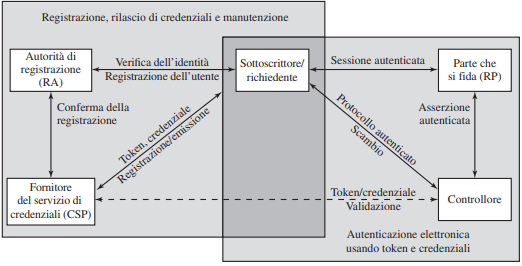
\includegraphics[width=\linewidth]{sp800.png}
    \caption{Schema del modello}
\end{figure}

\noindent Procedimento di registrazione:
\begin{enumerate}
    \item Il richiedente si rivolge a RA per diventare sottoscrittore in CSP
    \item Scambio di informazioni tra CSP e richiedente
    \item CSP rilascia una credenziale elettronica al richiedente (diventa sottoscrittore)
    \item Il sottoscrittore può adesso autenticarsi\newline
\end{enumerate}

\df{Il verificatore è un insieme di sistemi che effettuano autenticazione e autorizzazione}

\noindent Procedimento di autenticazione (previa registrazione):
\begin{enumerate}
    \item Il richiedente fa richiesta al verificatore
    \item Verifica tramite protocollo autenticativo
    \item Se OK il verificatore invia un'asserzione sull'identità a RP
    \item RP usa le informazioni per decidere accesso e autorizzazioni\newline
\end{enumerate}

\newpage

\subsection{Mezzi di autenticazione}

I mezzi principali per autenticare un utente sono 4:
\begin{enumerate}
    \item Qualcosa che conosce
    \item Qualcosa che possiede
    \item Qualcosa che è
    \item Qualcosa che ha\newline
\end{enumerate}

\df{L'autenticazione multifattore è l'uso di almeno 2 mezzi}

\subsubsection{Password}

Le password restano il metodo più diffuso, l'autenticazione avviene tramite la coppia (ID, password) presentata dall'utente al sistema. L'ID inoltre:
\begin{itemize}
    \item Determina se l'utente può accedere al sistema
    \item Determina i privilegi dell'utente
    \item Si usa nel controllo degli accessi discrezionale\newline
\end{itemize}

\noindent Solitamente le password non vengono salvate in chiaro, si salva l'hash (la funzione usata è volutamente lenta) (della password + un valore detto \textit{salt}) all'interno di un file che conterrà la riga (ID, salt, hash). Quando qualcuno deve autenticarsi si recupera nel file la riga corrispondente all'ID, si calcola l'hash con la password fornita ed il \textit{salt} salvato e se il risultato corrisponde a quello presente avviene l'autenticazione.\newline

\noindent Un tipo di attacco comune è il \textit{cracking} in cui si cerca di indovinare la password di un utente, tradizionalmente avviene in 2 modi:
\begin{enumerate}
    \item Si usa un dizionario contenente le password più comuni
    \item Si usa la \textit{Rainbow Table} che contiene gli hash precalcolati per ogni possibile \textit{salt}\newline
\end{enumerate}

\noindent Per cercare di rafforzare le password ma allo stesso tempo cercare di mantenerle memorizzabili ci sono diverse strategie:
\begin{itemize}
    \item Educare gli utenti
    \item Imporre delle regole sulla complessità
    \item Far generare le password al computer
    \item Mantenere un dizionario di password scadenti
    \item Effettuare un cracking "interno" per scovare le password deboli
    \item Usare il filtro di Bloom\newline

        Dato un dizionario delle password deboli. Un filtro di Bloom di ordine $k$ consiste in $k$ funzioni di hash indipendenti dove:
        
        $$H_i(x_j)=y \text{ con }1\leq i\leq k,\ 1\leq j\leq D,\ 0\leq y\leq N-1 $$

        In cui:
        \begin{itemize}
            \item $x_j$ è la $j$-esima parola nel dizionario
            \item $D$ è il numero di parole nel dizionario
            \item $N$ è un certo valore
        \end{itemize}

        Funzionamento:
        \begin{enumerate}
            \item Si definisce un'array di $N$ bit impostati a 0
            \item Per ogni password nel dizionario si calcolano i $k$ valori e usandoli come indici si settano a 1 quei bit nell'array
        \end{enumerate}

        Se viene presentata una nuova password e tutti i suoi valori di hash conducono a bit dell'array con valore 1 viene rifiutata. C'è comunque una possibilità di falsi positivi che si approssima con:

        $$\left(1-e^{-(kD)/N}\right)^k$$\newline

        Questo metodo permette di avere un dizionario enorme senza necessità di mantenerlo in memoria, inoltre velocizza il processo di controllo delle nuove password.\newline
    
\end{itemize}

\subsubsection{Biometria}

I sistemi biometrici sono basati sulle caratteristiche fisiche uniche degli utenti, alcune sono:
\begin{itemize}
    \item Impronte digitali
    \item Geometria della mano
    \item Schema della retina
    \item Firma
    \item Voce
\end{itemize}

\newpage

\noindent Funzionamento:

\begin{figure}[ht]
    \centering
    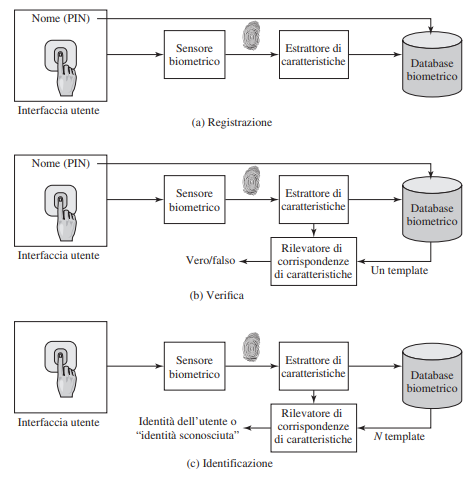
\includegraphics[width=0.8\linewidth]{biom.png}
\end{figure}

\noindent Come si può vedere può funzionare sia in modo simile alla password (Verifica) sia da solo (Identificazione).\newline

\noindent Essendo le caratteristiche fisiche molto complesse non ci si aspetta che ci sia una corrispondeza perfetta con la loro rappresentazione digitale, quindi si usano degli algoritmi che forniscono un punteggio di somiglianza tra il modello presentato e quello salvato. Questo ovviamente porta a falsi positivi/negativi.\newline

\begin{figure}[ht]
    \centering
    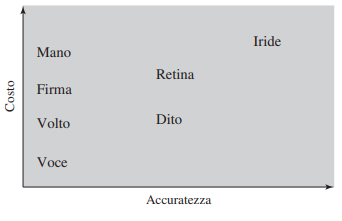
\includegraphics[width=0.55\linewidth]{acc.png}
\end{figure}

\section{Controllo degli accessi}

\df{Il controllo degli accessi è quel processo con cui si concede/nega una richiesta riguardante l'ottenimento/uso di informazioni e relativi servizi o si permette di far entrare un individuo in una struttura}

\df{L'autorizzazione è la concessione di un diritto/permesso ad un'entità di accedere ad una risorsa}

\df{Il controllo è la revisione/verifica delle attività e dei registri di sistema}

\df{CUI = informazioni non classificate controllate}

\noindent Un modello per rappresentare il procedimento è l'SP800-171:

\begin{table}[ht]
    \centering
    \begin{tabular}{|c|}
        \hline
        \textbf{Requisiti base}\\
        \hline
        Limitare l'accesso ai soli utenti autorizzati, i loro processi o i loro dispositivi\\
        \hline
        Limitare l'accesso ai tipi di transazioni/funzioni in base alle autorizzazioni dell'utente\\
        \hline
        \textbf{Requisiti derivati}\\
        \hline
        Controllare il flusso di CUI in base alle autorizzazioni\\
        \hline
        Separare i compiti degli individui\\
        \hline
        Usare il principio del minimo privilegio\\
        \hline
        Usare account/ruoli non privilegiati per funzioni non di sicurezza\\
        \hline
        Impedire agli utenti "normali" di usare funzioni privilegiate\\
        \hline
        Limitare i tentativi di accesso non riusciti\\
        \hline
        Fornire avvisi su Privacy e sicurezza in base alle norme in vigore\\
        \hline
        Interrompere le sessioni in caso di inattività prolungata\\
        \hline
        Terminare una sessione in presenza di certe condizioni\\
        \hline
        Controllare le sessioni remote\\
        \hline
        Usare la crittografia nelle sessioni remote\\
        \hline
        Indirizzare l'accesso remoto a dei punti di controllo\\
        \hline
        Autorizzare l'esecuzione remota di comandi privilegiati\\
        \hline
        Autorizzare l'accesso wireless prima di accettare le connessioni\\
        \hline
        Usare crittografia e autenticazione per gli accessi wireless\\
        \hline
        Controllare le connessioni mobili\\
        \hline
        Cifrare le CUI sui dispositivi mobili\\
        \hline
        Verificare/controllare/limitare le connessioni esterne\\
        \hline
        Limitare l'uso di dispositivi di archiviazione interni su sistemi esterni\\
        \hline
        Controllare le CUI sui sistemi accessibili al pubblico\\
        \hline
    \end{tabular}
    \caption{Requisiti del modello}
\end{table}

\df{Una politica di controllo definisce i tipi di accesso consentiti in quali condizioni e da chi}

\subsection{Discrezionale}

Il metodo tradizionale, si basa su 3 elementi:
\begin{enumerate}
    \item \textbf{Soggetto}
    \item \textbf{Oggetto}
    \item \textbf{Permesso d'accesso}
\end{enumerate}

\noindent Questi vengono organizzati in una matrice in cui le colonne sono gli oggetti, le righe i soggetti e le singole celle contengono i permessi del soggetto sull'oggetto.\newline

\begin{figure}[ht]
    \centering
    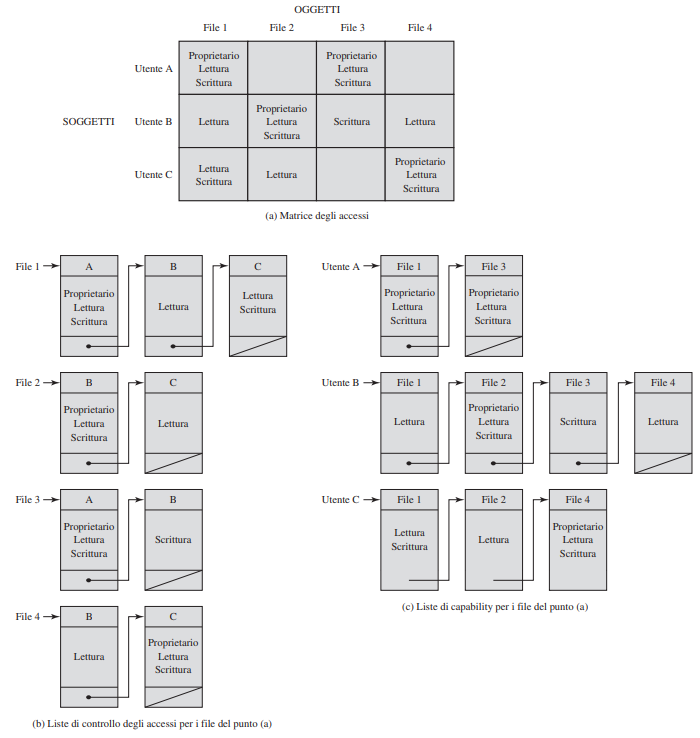
\includegraphics[width=0.91\linewidth]{dac.png}
    \caption{Esempio con file}
\end{figure}

\noindent La decomposizione per colonne fornisce le liste d'accesso dei file, quella per righe le capability list degli utenti.

\newpage

\noindent Un'alternativa è la tabella delle autorizzazioni:

\begin{table}[ht]
    \centering
    \begin{tabular}{c|c|c}
        Soggetto & Modalità d'accesso & Oggetto\\
        \hline
        A & Proprietario & F1\\
        \hline
        A & Scrittura & F3\\
        \hline
        B & Lettura & F3\\
    \end{tabular}
\end{table}

\noindent Il tutto si può estendere anche ad altri elementi:
\begin{itemize}
    \item \textbf{Processi} (Cancellarli, bloccarli, riattivarli)
    \item \textbf{Dispositivi} (Lettura, scrittura, controllo)
    \item \textbf{Locazioni/Regioni di memoria} (Lettura, scrittura)
    \item \textbf{Soggetti} (Cancellare, concedere permessi)
\end{itemize}
\noindent Ottenendo così una matrice estesa, per eseguire l'effettivo controllo è presente un controllore per ogni tipo di oggetto che usa le Entry della matrice per decidere:

\begin{figure}[ht]
    \centering
    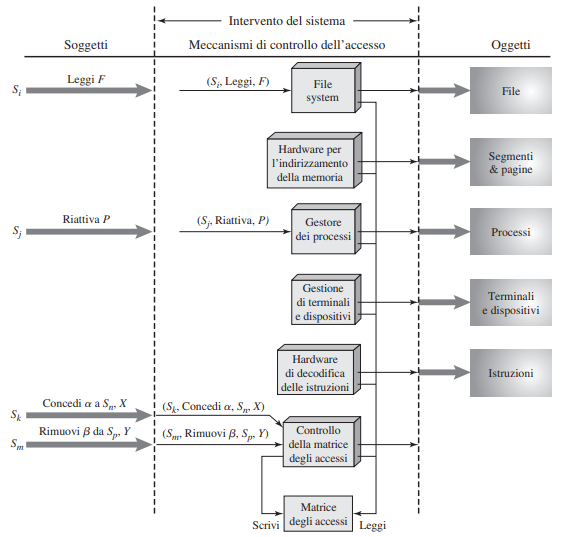
\includegraphics[width=0.92\linewidth]{contr.png}
    \caption{Esempio di funzionamento}
\end{figure}

\subsection{Basato su ruoli}

Questo sistema si basa sui ruoli che gli utenti possono assumere in un certo sistema (tipicamente con ruolo si intende una funzione lavorativa in un'organizzazione), l'assegnazione di questi ruoli avviene in modo dinamico mentre i ruoli tendono ad essere statici.\newline

\noindent Una famiglia di modelli è la seguente:
\begin{itemize}
    \item $RBAC_0$
    
        Contiene:
        \begin{itemize}
            \item \textbf{Utenti}
            \item \textbf{Ruoli}
            \item \textbf{Permessi} (associati ai ruoli)
            \item \textbf{Sessione} (mappatura tra utente e sottoinsieme dei suoi ruoli)
        \end{itemize}
    \item $RBAC_1$

        Come il precedente ma si aggiunge una gerarchia tra i ruoli usando l'ereditarietà.

    \item $RBAC_2$

        Come $RBAC_0$ ma con l'aggiunta di vincoli:
            \begin{itemize}
                \item \textbf{Cardinalità}, max utenti con certo ruolo
                \item \textbf{Mutua esclusività}, un utente non può avere più di 2 ruoli esclusivi contemporaneamente
                \item \textbf{Prerequisiti}, un utente ha un ruolo $x$ solo se ha anche il ruolo $y$
            \end{itemize}
    
    \item $RBAC_3$

        Unione di $RBAC_1$ e $RBAC_2$.\newline
    
\end{itemize}

\noindent In breve:\newline

\begin{table}[ht]
    \centering
    \begin{tabular}{c|c|c}
        Modello & Gerarchia & Vincoli\\
        \hline
        $RBAC_0$ &  & \\
        \hline
        $RBAC_1$ & x & \\
        \hline
        $RBAC_2$ &  & x\\
        \hline
        $RBAC_3$ & x & x\\
    \end{tabular}
\end{table}

\noindent Anche in questo caso si possono usare le matrici, una per associare i permessi ai ruoli e un'altra per associare i ruoli agli utenti.

\subsection{Basato su attributi}

Un attributo rappresenta una certa caratteristica di soggetti, oggetti e condizioni ambientali, per controllare gli accessi vengono presi in considerazioni gli attributi di tutti e 3 gli elementi:

\begin{figure}[ht]
    \centering
    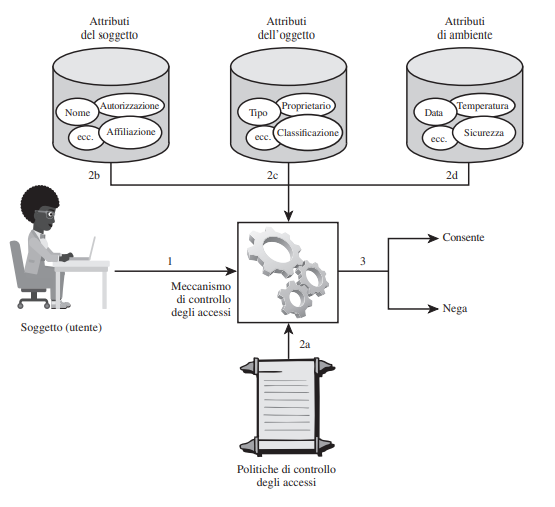
\includegraphics[width=0.82\linewidth]{abac.png}
    \caption{Funzionamento}
\end{figure}

\noindent\rule{\textwidth}{0.5pt}
\noindent Esempio:

\begin{table}[ht]
    \centering
    \begin{tabular}{c|c}
        Classificazione Film & Età minima\\
         \hline
        R & 17\\
         PG-13& 13\\
        G & -\\
    \end{tabular}
\end{table}

\noindent Agli utenti viene assegnato un attributo riguardante la loro età durante la registrazione, per garantire che un utente acceda ad un film solo se ha almeno l'età minima basta una sola regola (ignorando l'ambiente):

\begin{equation}
    \nonumber
    \begin{split}
        R1:can\_access(u,m,e)\leftarrow\  & (Age(u)\geq17\wedge Rating(m)\in\{R,PG-13,G\})\ \vee \\
        & (Age(u)\geq13\wedge Rating(m)\in\{PG-13,G\})\ \vee\\
        & (Age(u)<13\wedge Rating(m)\in\{G\})
    \end{split}
\end{equation}

\noindent\rule{\textwidth}{0.5pt}

\section{Database}

\subsection{SQL Injection}

Si tratta di attacchi progettati per estrarre/cancellare/modificare dei dati in un DB, solitamente sfruttano l'interazione tra il DB e le pagine web per inserire istruzioni malevole.\newline

\noindent L'attacco consiste nell'inserimento di specifiche stringhe che vanno a modificare la Query costruita nel back-end, così facendo è possibile prelevare informazioni che normalmente dovrebbero essere private.\newline

\noindent Esistono diversi modi per inviare le istruzioni:
\begin{itemize}
    \item Input utente
    \item Variabili del server
    \item Cookie
    \item Input fisici\newline
\end{itemize}

\noindent E diversi tipi di attacchi:
\begin{itemize}
    \item In banda (stesso canale per invio e ricezione)
        \begin{itemize}
            \item \textbf{Tautologia}

                Uso di istruzioni condizionali sempre vere.
            
            \item \textbf{Commento a fine riga}

                Inserimento di '- -' a fine riga, tutto ciò che viene dopo diventa un commento.
            
            \item \textbf{Query Piggybacked}

                Concatenazione di una Query a quella leggittima.
            
        \end{itemize}

    \item Fuori banda (canali diversi)

    \item Inferenziale (ricostruzione delle informazioni)
        \begin{itemize}
            \item \textbf{Query illecite/sbagliate}

                Ricavo di informazioni dalla pagina di errore.
            
            \item \textbf{Blind SQL}

                Invio di Query di tipo Vero/Falso ed analisi dei risultati.\newline
            
        \end{itemize}
\end{itemize}

\df{L'inferenza è un processo che consiste nell'effettuare richieste leggittime e dedurre informazioni riservate partendo dai risultati ottenuti}

\newpage

\noindent Le principali contromisure sono:
\begin{itemize}
    \item Programmazione difensiva
            \begin{itemize}
                \item \textbf{Pratiche manuali}

                    Controllo del tipo di dato, riconoscimento sequenze anomale.
                
                \item \textbf{Inserimento parametrizzato}

                    Definizione dettagliata della Query, inserimento sequenziale dei parametri. 
                
                \item \textbf{SQL DOM}

                    Insieme di classi per la validazione automatica.
                
            \end{itemize}
    \item Rilevazione
        \begin{itemize}
            \item \textbf{Su firma}

                Individuazione delle specifiche sequenze di attacco.
            
            \item \textbf{Su anomalia}

                Definizione di modello comportamentale, individuazione di attività che si discostano da esso.
            
            \item \textbf{Analisi del codice}

                Uso di specifici test per rilevare le vulnerabilità.
            
        \end{itemize}
    \item Prevenzione a Run-time

        Controllo delle Query a run-time con appositi strumenti.
    
\end{itemize}

\subsection{Controllo degli accessi}

I DBMS implementano dei sistemi di controllo discrezionali e a ruoli, e si basano sul presupposto che il sistema autentichi ogni singolo utente.\newline

\noindent Lo stesso linguaggio SQL ha 2 comandi che permettono di concedere/revocare ruoli agli utenti e permessi ai ruoli:
\begin{itemize}
    \item $GRANT$
    \item $REVOKE$\newline
\end{itemize}

\noindent Scegliendo alcune opzioni è possibile usarli in cascata, nel caso della revoca ad un utente che ha ricevuto lo stesso permesso da più utenti si segue la regola "\textit{Quando un utente revoca un permesso verrano revocati tutti a cascata, a meno che un certo permesso sarebbe esistito anche se l'utente non avesse concesso il permesso}".

\newpage

\subsection{Cifratura}

La cifratura rappresenta l'ultimo sistema di difesa per un DB, essa può essere applicata a diversi "livelli" (attributi, record, campi, $\ldots$), porta però a 2 problemi:
\begin{enumerate}
    \item \textbf{Gestione delle chiavi}

        Ogni utente deve conoscere la chiave per accedere ai dati e gli utenti interessati possono essere molti.
    
    \item \textbf{Rigidità}

        La ricerca dei dati diventa più complessa.\newline

\end{enumerate}

\begin{figure}[ht]
    \centering
    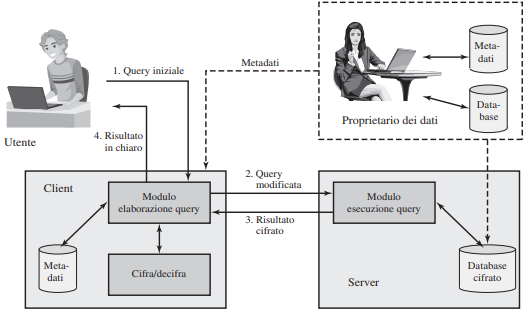
\includegraphics[width=\linewidth]{db.png}
    \caption{Funzionamento}
\end{figure}

\noindent Le 2 opzioni principali sono:
\begin{enumerate}
    \item \textbf{Cifrare tutto}
    \item \textbf{Cifrare i record}

        Ogni riga viene cifrata come fosse un blocco unico e vengono aggiunti degli indici per gli attributi (non necessariamente tutti) [$E(k,(x_1|x_2|\ldots)),I_1,I_2,\ldots$]

        \vspace{3pt}
        
        Gli indici servono per semplificare la ricerca, i valori assumibili da essi rappresentano ognuno un sottointervallo dei valori assumibili da quell'attributo, ovviamente il valore che assume in una riga dipende dal valore di quell'attributo nella stessa.
    
\end{enumerate}

\section{Software malevolo}

\df{Un malware è un programma che viene inserito in un sistema (solitamente di nascosto) con l'intento di compromettere il sistema stesso o i suoi dati}

\df{Un kit di attacco è un insieme di strumenti che può generare automaticamente malware}

\df{Un ATP è un tipo di attacco che si distingue dagli altri per la sua selezione accurata del bersaglio e la sua persistenza nel tempo}

\df{Il payload sono le azioni malevole che svolge un malware}

\subsection{Virus}

\df{Un Virus è un frammento software che infetta altri programmi inserendo in essi del codice che generi delle copie di sè stesso}

\noindent Solitamente è inserito in un programma e viene eseguito ogni volta che si esegue il programma relativo operando con i suoi privilegi. Gli elementi costitutivi sono:
\begin{itemize}
    \item \textbf{Vettore di infezione}
    \item \textbf{Trigger}
    \item \textbf{Payload}\newline
\end{itemize}

\noindent Attraversa 4 fasi durante la sua vita:
\begin{enumerate}
    \item \textbf{Dormiente}
    \item \textbf{Propagazione}
    \item \textbf{Attivazione}
    \item \textbf{Esecuzione}\newline
\end{enumerate}

\noindent Si può dare una classificazione per target:
\begin{itemize}
    \item \textbf{Boot Sector infector}
    \item \textbf{File infector}
    \item \textbf{Macro Virus}
    \item \textbf{Virus multipartito}
\end{itemize}

\noindent Ed una in base al camuffamento usato:
\begin{itemize}
    \item \textbf{Criptato}
    \item \textbf{Furtivo}
    \item \textbf{Polimorfo}

        Le sue copie hanno stesse funzioni ma pattern diversi.
    
    \item \textbf{Metamorfico}

        Ad ogni iterazione si ridefinisce totalmente.\newline
    
\end{itemize}

\noindent In particolare i Macro Virus si "attaccano" ai documenti e sfruttano le operazioni Macro delle applicazioni apposite, questo li rende indipendenti dalla piattaforma e facilmente creabili.\newline

\subsection{Worm}

\df{Un Worm è un programma che cerca attivamente nuovi sistemi da infettare, sfrutta quelli già infetti come "trampolino di lancio"}

\noindent I principali mezzi usati sono:
\begin{itemize}
    \item E-mail
    \item Chat istantanee
    \item MMS
    \item Bluetooth
    \item Condivisione file
    \item Trasferimento/Accesso remoto\newline
\end{itemize}

\noindent Le sue fasi sono simili a quelle del virus, nel dettaglio la propagazione tramite rete prevede 4 possibili strategie:
\begin{itemize}
    \item \textbf{Casuale}

        Prova tutti i possibili indirizzi.
    
    \item \textbf{Hit-list}

        Redige una lista dei possibili bersagli.
    
    \item \textbf{Topologica}

        Sfrutta le informazioni della macchina.
    
    \item \textbf{Sottorete locale}

        Sfrutta la struttura della sottorete se riesce ad attraversare il firewall.
    
\end{itemize}

\newpage

\noindent Un fatto importante è che la sua percentuale di diffusione presenta delle similitudini con i virus biologici, l'andamento si può esprimere con la formula:
$$\frac{d\ I(t)}{d\ t}=\beta I(t)S(t)$$
\noindent In cui:
\begin{itemize}
    \item \textcolor{ForestGreen}{$I(t)$ è il numero di individui infetti al tempo $t$}
    \item \textcolor{Blue}{$S(t)$ è il numero di individui suscettibili all'infezione al tempo $t$}
    \item $\beta$ è il tasso di infezione
    \item $N=I(t)+S(t)$ è la dimensione della popolazione\newline
\end{itemize}

\begin{figure}[ht]
    \centering
    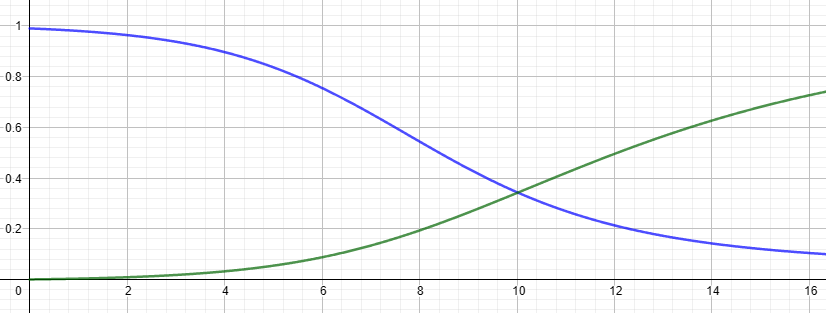
\includegraphics[width=\linewidth]{worm.png}
    \caption{Esempio di andamento}
\end{figure}

\vspace{5pt}

\df{Il mobile code è l'insieme di programmi che possono essere trasmessi invariati ad un insieme eterogeneo di piattaforme con la stessa semantica}

\noindent Alcuni metodi di diffusione più specifici sono:
\begin{itemize}
    \item \textbf{Drive-by-download}

        Exploit di bug nelle applicazioni utente per installare malware, per esempio un sito web che scarica un file senza il consenso.
    
    \item \textbf{Watering-hole}

        Versione mirata del precedente, è preceduto da uno studio della vittima. In alcuni casi si sfrutta il Malvertising.
    
    \item \textbf{Clickjacking}

        Acquisizione dei click, forza l'utente a svolgere certe azioni.
        
\end{itemize}

\subsection{Trojan}

\df{Un Trojan è un/una programma/procedura in apparenza utile che contiene codice malevolo nascosto}

\noindent I modelli principali sono 3:
\begin{enumerate}
    \item Svolge sia la funzione normale che quella malevola
    \item Svolge la funzione normale ma essa viene modificata
    \item Sovverte completamente la funzione normale\newline
\end{enumerate}

\noindent Il loro mezzo di diffusione principale è lo Spam di e-mail, con l'ascesa dei telefoni cellulari però si è iniziato a diffonderli tramite i Marketplace delle applicazioni. I Trojan per smartphone risultano estremamente dannosi data la presenza di molte informazioni personali su di essi.\newline

\subsection{Payload}

I principali tipi di Payload sono:
\begin{itemize}

    \item \textbf{Ransomware}

        Criptano i dati del sistema e chiedono un riscatto per la chiave.

    \item \textbf{Distruzione dati}

    \item \textbf{Distruzione apparecchiature fisiche}

    \item \textbf{Creazione zombie/bot/droni}

        Essi sono sistemi infetti le cui risorse vengono usate per lanciare attacchi, i principali sono:
            \begin{itemize}
                \item DDOS
                \item Spamming
                \item Sniffing del traffico
                \item Keylogging
                \item Diffusione malware
            \end{itemize}

    \item \textbf{Keylogging}

        Lettura dei tasti premuti dall'utente.

    \item \textbf{Creazione Backdoor}

    \item \textbf{Creazione Rootkit}

        Come il precedente ma mantiene l'accesso con privilegi di amministratore.
    
\end{itemize}

\subsection{Contromisure}

Il metodo migliore per contrastare la diffusione dei malware resta la prevenzione, le misure sono piuttosto semplici:
\begin{itemize}
    \item Avere i sistemi sempre aggiornati
    \item Controllare gli accessi ad applicazioni e dati
    \item Sensibilizzare gli utenti\newline
\end{itemize}

\noindent Nel caso non basti si cerca di mitigare i danni:
\begin{itemize}
    \item Eliminare i file infetti
    \item Usare i backup
    \item Cancellazione completa e successivo ripristino (in extremis)\newline
\end{itemize}

\noindent A livello dei singoli dispositivi si fa uso di Antivirus, esistono diverse generazioni:
\begin{enumerate}
    \item Identificazione con firma
    \item Uso di criteri euristici e controllo integrità dei programmi
    \item Analisi dinamica
    \item Combinazione dei precedenti\newline
\end{enumerate}

\noindent Un tipo di analisi particolare è quella Sandbox, essa consiste nell'eseguire il codice in ambiente controllato (VM, emulatori) e monitorare l'andamento.\newline

\noindent A livello di rete invece si usa una scansione perimetrale:
\begin{itemize}
    \item Monitor di ingresso (tra rete interna ed internet)
        \begin{itemize}
            \item Ricerca firme
            \item Honeypot
        \end{itemize}
    \item Monitor di uscita (tra sottoreti)
    \begin{itemize}
        \item Controllo traffico in uscita
        \item "Data-loss"\newline
    \end{itemize}
\end{itemize}

\noindent Il metodo migliore è una combinazione dei due, definendo un sistema centrale dedito all'analisi la rete diventa simile ad un sistema immunitario. 

\section{DOS}

\df{Un attacco DOS previene/incapacita l'uso di reti/sistemi/applicazioni esaurendo le loro risorse}

\df{DDOS = attacco DOS distribuito, solitamente tramite net-bot}

\noindent I tipi principali sono:
\begin{itemize}
    \item \textbf{Flooding}

        Il metodo più semplice, si inviano una grande quantità di pacchetti al bersaglio.
    
    \item \textbf{Spoofing indirizzo}

        Vengono "forgiati" degli indirizzi IP e poi usati nei pacchetti, rende il rintracciamento più difficile. 
    
    \item \textbf{Spoofing Syn}

        Come il precedente ma il bersaglio è la tabella delle connessioni TCP, si cerca di mantenerla sempre piena per non permettere nuove connessioni. Dato il funzionamento di TCP l'uso di indirizzi non esistenti genera ulteriore traffico che va a congestionare ulteriormente la rete.
     
    \item \textbf{VoIP}

        Sfrutta le richieste \textit{INVITE} (dispendiose a livello di risorse) del protocollo SIP, un flooding di queste richieste non permette al bersaglio di ricevere telefonate.
    
    \item \textbf{HTTP}

        Ci sono 2 varianti non banali:
            \begin{enumerate}
                \item \textbf{Spidering}

                    Si tratta di un flood di richieste HTTP ricorsivo, opera su una pagina e i link presenti in essa ricorsivamente.
                
                \item \textbf{Slowrolis}

                    Cerca di mantenere la connessione con il server aperta per più tempo possibile, fa ciò inviando inizialmente una richiesta parziale e successivamente linee di header incomplete in modo periodico senza però finire mai la richiesta.
                
            \end{enumerate}
    
    \item \textbf{Di riflesso}

        Usando l'IP del bersaglio si fanno richieste continue ad un intermediario che invierà i risultati al destinatario.
    
    \item \textbf{Di amplificazione}

        Come il precedente ma si usano indirizzi di intere reti per generare ancora più traffico.
    
\end{itemize}

\subsection{Difesa}

\noindent Le linee di difesa sono 4:
\begin{enumerate}
    \item Prevenire gli attacchi
    \item Filtrare il traffico
    \item Identificare la sorgente
    \item Eliminare gli effetti dell'attacco\newline
\end{enumerate}

\noindent Per prevenire ci sono diversi modi:
\begin{itemize}
    \item Limitare l'uso di indirizzi "forgiati"
    \item Assicurarsi che la via di ritorno del pacchetto sia quella giusta
    \item Limitare la quantità di certi tipi di pacchetti
    \item Gestire in modo diverso le connessioni TCP
    \item Bloccare gli indirizzi di broadcast
    \item Usare i Captcha
    \item Usare server specchiati/replicati\newline
\end{itemize}

\noindent In ogni caso bisogna definire un piano di risposta:
\begin{enumerate}
    \item Come contattare il personale ISP senza la rete
    \item Imporre un filtraggio del traffico
    \item Come rispondere\newline
\end{enumerate}

\noindent In particolare:
\begin{itemize}
    \item Identificare il tipo di attacco
    \item Cercare di identificare la sorgente
    \item In caso di attacco duraturo avere un piano di contingenza
    \item Aggiornare continuamente il piano di risposta\newline
\end{itemize}

\section{Rilevamento intrusioni}

I sistemi di rilevamento intrusioni sono composti da:
\begin{itemize}
    \item Sensori
    \item Analizzatori
    \item Interfaccia grafica\newline
\end{itemize}

\noindent Sono basati sul fatto che il comportamento di un utente legittimo differisce da quello di un attaccante, è comunque presente un certo grado di incertezza che può portare a falsi rilevamenti.\newline

\begin{table}[ht]
    \centering
    \begin{tabular}{c|c|c}
        Esecuzione continua & Tolleranza ai guasti & Resistenza alla sovversione\\
         \hline
        Overhead minimo & Configurazione con \textit{policies} & Adattamento ai cambiamenti\\
         \hline
        Scalabilità & Degradazione graziosa & Riconfigurazione dinamica\\
    \end{tabular}
    \caption{Requisiti IDS}
\end{table}

\noindent Funzionamento:
\begin{enumerate}
    \item Creazione del modello comportamentale

        3 metodi:
            \begin{enumerate}
                \item \textbf{Statistico}

                    Uso di modelli univariati/multivariati/a serie di tempo.
                
                \item \textbf{Basato su conoscenza}

                    Si usa un sistema esperto basato su certe regole.
                
                \item \textbf{Basato su Machine Learning}

                    Ci sono molti modi:
                        \begin{itemize}
                            \item Reti Bayesiane
                            \item Logica Fuzzy
                            \item Reti neurali
                            \item Algoritmi genetici
                            \item $\ldots$
                        \end{itemize}
                
            \end{enumerate}
    
    \item Rilevazione
        \begin{itemize}
            \item \textbf{Euristica}

                Si usano delle regole prefissate.
            
            \item \textbf{Con firma}

                Si comparano i pattern conosciuti con quelli presenti in un sistema o transitanti sulla rete.\newline
            
        \end{itemize}
    
\end{enumerate}

\subsection{Tipi}

\noindent In base a dove operano si distinguono:
\begin{itemize}
    \item \textbf{HIDS} (host)

        Possibili sorgenti di dati sono:
        \begin{itemize}
            \item Chiamate di sistema
            \item Log file
            \item Checksum d'integrità
            \item Accessi ai registri (Windows)
        \end{itemize}

        Nelle LAN si possono creare dei sistemi HIDS distribuiti, alcuni nodi fungeranno da punti di raccolta ed analisi dati. 
    
    \item \textbf{NIDS} (rete)

        2 tipi:
        \begin{enumerate}
            \item \textbf{Inline}

                Dei veri e propri nodi, il traffico li attraversa.
            
            \item \textbf{Passivi}

                Ricevono una copia del traffico.
            
        \end{enumerate}

        Solitamente i punti in cui si inseriscono sono:
        \begin{itemize}
            \item Sul Firewall esterno
            \item Tra Firewall esterno ed Internet
            \item Tra LAN e rete interna
            \item Tra Backbone e rete interna
        \end{itemize}
    
    \item \textbf{IDS ibridi/distribuiti}

        Quando i singoli nodi rilevano dell'attività sospetta fanno "gossip" agli altri nodi, se un nodo ne riceve una quantità considerevole presume ci sia un attacco e risponde di conseguenza.\newline
    
\end{itemize}

\noindent\textbf{Definizione} Gli Honeypot sono sistemi esca creati appositamente per adescare gli attaccanti, hanno il compito di deviare gli attacchi lontano dai sistemi critici e allo stesso tempo incoraggiare gli attaccanti a restare più tempo possibile. Per fare ciò contengono delle informazioni fabbricate e fanno in modo che ogni attacco verso di loro vada sempre a buon fine.\newline

\noindent Ce ne sono 2 tipi:
\begin{enumerate}
    \item \textbf{A bassa interazione}

        Pacchetti software che emulano servizi/sistemi in modo realistico.
    
    \item \textbf{Ad alta interazione}

        Sistemi veri e propri.
    
\end{enumerate}

\section{Firewall}

\noindent\textbf{Definizione} Il Firewall è un componente hardware/software inserito tra la rete interna ed internet, funziona essenzialmente da filtro.\newline

\noindent I tipi principali sono 4:
\begin{enumerate}
    \item \textbf{A filtro di pacchetti}

        Si basa su delle regole riguardanti i campi dei pacchetti, in particolare:
        \begin{itemize}
            \item IP sorgente/destinazione
            \item Porta sorgente/destinazione
            \item UDP/TCP
            \item Interfaccia in/out
        \end{itemize}

    \item \textbf{Con filtraggio stateful}

        Mantiene una tabella delle connessioni TCP in uscita, permette ai pacchetti di entrare solo se riguardanti una connessione attiva.

    \item \textbf{Gateway di applicazione}

        Fa da relay per per il traffico a livello applicativo, segue questo procedimento:
            \begin{enumerate}
                \item Utente chiede servizio al Firewall
                \item Firewall chiede l'Host a cui accedere
                \item L'Utente invia il nome dell'Host
                \item L'utente fornisce il suo ID e le informazioni di autenticazione
                \item Il Firewall contatta l'Host e poi inizia a trasmettere
            \end{enumerate}

    \item \textbf{Gateway di circuito}

        "Spezza" le connessioni TCP in 2 e fa da intermediario: 
        $$\text{Host interno} \longleftrightarrow^{TCP} \text{Firewall} \longleftrightarrow^{TCP} \text{Host esterno}$$\newline
    
\end{enumerate}

\noindent In base al posizionamento si identificano:
\begin{itemize}
    \item \textbf{Bastion Host}

        Si trova in un punto critico per la rete.
    
    \item \textbf{Host-based}

        Posto su i singoli host, solitamente sui server.
    
    \item \textbf{Personali}

        Si trova sui PC "personali".

\end{itemize}

\newpage

\noindent Usando 2 firewall (interno ed esterno) è possibile creare una DMZ in cui sono presenti i dispositivi che devono essere protetti ma allo stesso tempo devono essere accessibili dall'esterno.\newline

\noindent\textbf{Definizione} Un VPN è un insieme di PC connessi tramite una rete non sicura che usano cifratura ed appositi protocolli per comunicare in modo sicuro, questo lavoro viene svolto solitamente tramite software dai router o dai firewall.\newline

\section{Buffer Overflow}

\df{Il buffer overflow è una condizione d'errore in cui vengono scritti in un buffer più dati di quanti ne possa contenere}

\noindent Solitamente si verifica a causa di un errore di programmazione, considerando inoltre che il buffer si trova nell'Heap/Stack/Sezione dati del programma c'è il rischio che gli elementi vicino ad esso vengano modificati.\newline

\noindent Nel caso il buffer si trovi nella stack l'attacco classico punta a modificare l'indirizzo di ritorno nello stack frame, il modo più semplice è inserire una quantità di dati nel buffer tale che essi vadano a "risalire" fino all'indirizzo e modificarlo. Generalmente questo porta ad un crash del programma, in casi più sofisticati si inserisce nel buffer la "traduzione" di codice macchina insieme ad un \textit{NOP-SLED} e si cerca di modificare l'indirizzo facendolo puntare al codice inserito per eseguirlo.\newline

\noindent Alcuni metodi per prevenirlo sono:
\begin{itemize}
    \item Scegliere un linguaggio di programmazione adatto
    \item Scrivere codice sicuro
    \item Usare meccanismi di protezione della stack
    \item Usare delle pagine di guardia
    \item Proteggere lo spazio degli indirizzi
    \item Randomizzare lo spazio degli indirizzi
\end{itemize}

\newpage

\vspace*{-3\baselineskip}

\section{Sicurezza del software}

Nel mondo del Software ci sono 3 principali elementi che portano a degli errori:
\begin{enumerate}
    \item Interazione non sicura tra i componenti
    \item Gestione non oculata delle risorse
    \item Difese deboli\newline
\end{enumerate}

\df{La programmazione difensiva è il processo di programmazione e implementazione che garantisce il funzionamento del programma anche sotto attacco, esso deve continuare la sua esecuzione o fallire elegantemente}

\begin{figure}[ht]
    \centering
    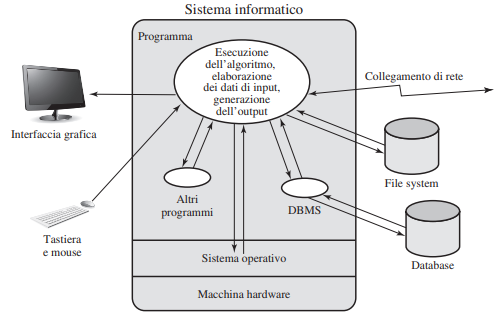
\includegraphics[width=0.8\linewidth]{prog.png}
    \caption{Modello di un programma}
\end{figure}

\noindent Gli elementi chiave da gestire sono:
\begin{itemize}
    \item Codice stesso
    
        Implementare correttamente gli algoritmi, gestire opportunamente la memoria e interpretare correttamente i valori usati.
    
    \item Interazione con altri programmi/S.O.

        Fornire i privilegi minimi possibili, prevenire le race condition e controllare le librerie usate.
    
    \item Input

        Controllare le dimensioni, il tipo e accertarsi che sia conforme.
    
    \item Output

        Filtrare i dati definendo quelli ammissibili ed accertarsi della loro conformità.
    
\end{itemize}

\section{Crittografia}

Uno schema di cifratura è computazionalmente sicuro se:
\begin{itemize}
    \item Il costo per rompere la cifratura è maggiore del valore delle informazioni cifrate
    \item Il tempo necessario per rompere la cifratura è maggiore della vita utile delle informazioni cifrate\newline
\end{itemize}

\subsection{Simmetrica}

Questo tipo necessita che la chiave usata sia uguale ai 2 capi della comunicazione, si distinguono:
\begin{itemize}
    \item \textbf{A blocchi} (DES,3DES,AES)

        Il messaggio viene diviso in blocchi che verranno poi cifrati ed inviati, sono presenti diversi modi per procedere:
        \begin{itemize}
            \item \textbf{ECB}

                Si usano blocchi da 64 bit.

                \begin{figure}[ht]
                    \centering
                    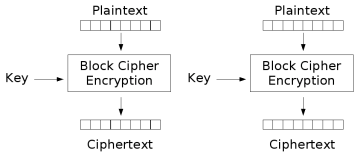
\includegraphics[width=0.6\linewidth]{ecb.png}
                \end{figure}

            \item \textbf{CBC}

                \begin{figure}[ht]
                    \centering
                    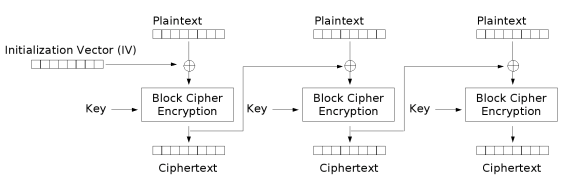
\includegraphics[width=0.9\linewidth]{cbc.png}
                \end{figure}

                Per riavere il blocco in chiaro si deve decifrare il blocco e poi fare lo $XOR$ con il blocco cifrato precedente.

            \newpage

            \item \textbf{CFB}

                Serve a trasformare la cifratura in blocchi in una cifratura di flusso.

                \begin{figure}[ht]
                    \centering
                    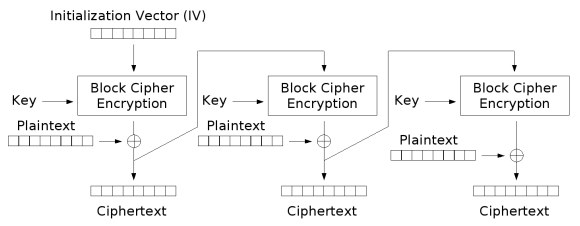
\includegraphics[width=0.9\linewidth]{cfb.png}
                \end{figure}                

            \item \textbf{OFB}

                Come il precedente ma l'input della prossima cifratura è preso prima dello $XOR$.\newline

            \item \textbf{CTR}

                Simile a ECB ma l'input della cifratura è un contatore incrementato ad ogni blocco ed il risultato è dato dallo $XOR$ dell'output e del blocco in chiaro.

                \begin{figure}[ht]
                    \centering
                    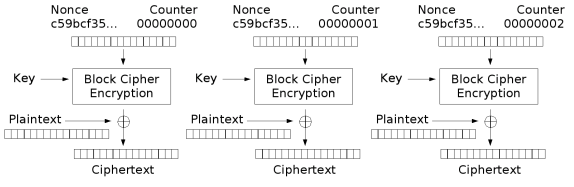
\includegraphics[width=0.9\linewidth]{ctr.png}
                \end{figure}                   
            
        \end{itemize}
    
    \item \textbf{Di flusso} (RC4)

        Viene usata per cifrare un flusso continuo di informazioni, gli elementi vengono dati in output uno alla volta.
    
\end{itemize}

\newpage

\subsubsection{DES e 3DES}

Questo schema è basato su una versione leggermente modificata della struttura di Feistel:

\begin{figure}[ht]
    \centering
    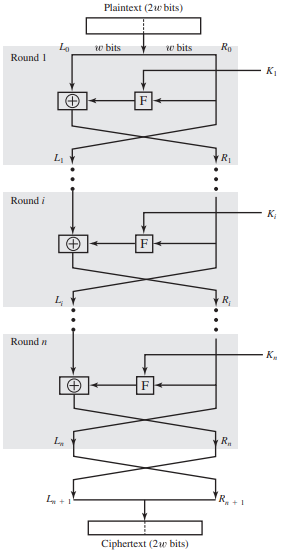
\includegraphics[width=0.5\linewidth]{feistel.png}
    \caption{Struttura di Feistel}
\end{figure}

\noindent In cui:
\begin{itemize}
    \item F è la funzione di round
    \item Le sottochiavi sono generate dalla chiave con una certa funzione\newline
\end{itemize}

\noindent In particolare usa:
\begin{itemize}
    \item Blocchi da 64 bit
    \item Chiave da 56 bit
    \item 16 round
\end{itemize}

\newpage

\noindent 3DES usa 3 chiavi ed applica DES 3 volte di fila nel seguente modo:

\begin{figure}[ht]
    \centering
    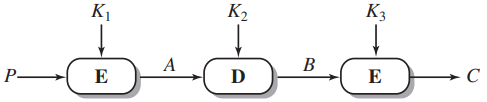
\includegraphics[width=0.65\linewidth]{3des.png}
\end{figure}

\subsubsection{AES}

\begin{figure}[H]
    \centering
    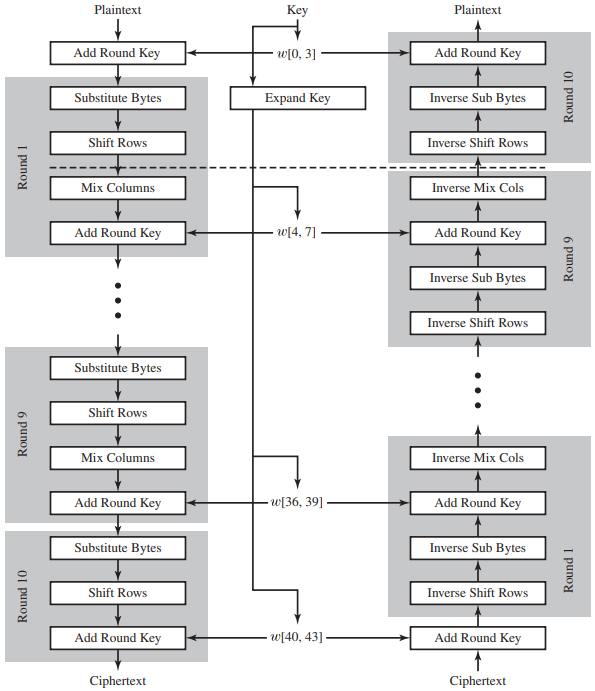
\includegraphics[width=0.8\linewidth]{aes.png}
    \caption{Funzionamento}
\end{figure}

\noindent Nel dettaglio:
\begin{itemize}
    \item Blocchi da 182 bit
    \item Chiave da 128/192/256 bit
    \item 10/12/14 round in base alla chiave

\newpage

    \item La chiave viene espansa tramite una funzione in un array lineare con grandezza dipendente dalla chiave, nei primi posti ci sarà la chiave stessa

    \item Il blocco viene copiato in un array detto stato su cui si eseguirà il procedimento e costituirà alla fine l'output

    \item \textbf{Substitute bytes}

        Si usa una \textit{S-Box} di $16\times16$ bit contenente una permutazione dei valori assumibili da un byte (256), usando i 4 bit a sx e dx dello stato si trova il nuovo valore che costituirà lo stato

    \item \textbf{Shift Row}

        Su ogni riga dello stato si fa uno shift a sx circolare di $n-1$ posizioni con $n$ numero di riga.

    \item \textbf{Mix columns}

        Ogni byte di ogni colonna ottiene un nuovo valore dato da tutti i byte presenti nella colonna stessa.

    \item \textbf{Add round key}

        $XOR$ tra stato e chiave di round (per colonna)
        
\end{itemize}

\subsubsection{RC4}

\begin{algorithm}[ht]
\caption{Generazione stream }
\begin{algorithmic}

\For{$i\in[0,255]$} \Comment{Inizializzazione}

    \State S[i] = i
    \State T[i] = key[i$\mod(len(key))$]

\EndFor

\State

\State j = 0 \Comment{Permutazione iniziale}

\For{$i\in[0,255]$} 

    \State j = (j+S[i]+T[i])$\mod(256)$
    \State Swap(S[i],S[j])

\EndFor

\State

\State i,j = 0 \Comment{Generazione stream}

\While{1}

    \State i = (i+1)$\mod(256)$
    \State j = (j+S[i])$\mod(256)$
    \State Swap(S[i],S[j])
    \State t = (S[j]+S[i])$\mod(256)$
    \State x = S(t)

\EndWhile

\end{algorithmic}
\end{algorithm}

\newpage

\noindent In breve:
\begin{itemize}
    \item La chiave ha lunghezza $[1,256]$ byte
\end{itemize}
\begin{enumerate}
    \item S contiene $[0,255]$
    \item T contiene la chiave intera o ripetuta
    \item S diventa una permutazione di se stesso
    \item Si itera sugli elementi in S ed in base alla sua configurazione si effettua lo Swap\newline
    
\end{enumerate}

\noindent Per cifrare basta fare lo $XOR$ tra $x$ ed il byte del testo in chiaro correnti, per decifrare basta rifare lo $XOR$ del byte cifrato corrente con $x$.

\subsection{Asimmetrica}

Si distinguono chiave pubblica e privata, con quella pubblica chiunque può cifrare un messaggio che potrà essere decifrato solamente con la chiave privata.

\subsubsection{RSA}

Il testo in chiaro $M$ ed il testo cifrato $C$ vengono visti come 2 interi tra 0 e $n-1$:
$$C=M^e\mod n$$
$$M=C^d\mod n=(M^e)^d\mod n=M^{ed}\mod n$$

\noindent Si devono soddisfare i seguenti requisiti:
\begin{itemize}
    \item Si possono trovare $e,d,n$ tali che $\forall\ M<n\ \ M^{ed}\mod n=M$
    \item $\forall\ M<n\ \ M^e,C^d$ sono facilmente calcolabili
    \item Non si può calcolare $d$ partendo da $e$ o $n$
\end{itemize}

\noindent La chiave pubblica sarà $\{e,n\}$ e quella privata $\{d,n\}$.\newline

\noindent Il primo punto tiene solo se $e,d$ sono inversi moltiplicativi modulo $\phi(n)$, quindi devono entrambi essere coprimi a $\phi(n)$.

\begin{algorithm}[ht]
\caption{Trovare le chiavi}
\begin{algorithmic}

\State Scegliere $p,q\ |\ p\neq q\wedge\text{ entrambi primi}$
\State $n=pq$
\State $\phi(n)=(p-1)(q-1)$
\State Selezionare $e\ |\ MCD(\phi(n),e)=1\wedge1<e<\phi(n)$
\State Calcolare $d$ sapendo che $de\mod\phi(n)=1$

\end{algorithmic}
\end{algorithm}

\subsubsection{Diffie-Hellman}

\noindent\textbf{Definizione} La radice primitiva di un numero primo $p$ è un numero $a$ tale che:
$$a\mod p,a^2\mod p,\ \ldots\ ,a^{p-1}\mod p $$

\noindent Sono tutti distinti e generano tutti i numeri da 1 a $p-1$.\newline

\noindent\textbf{Definizione} Dato $p$ ed $a$ sua radice primitiva. Per ogni $b<p$ si può trovare un numero $i$ detto logaritmo discreto per cui:
$$b=a^i\mod p\ \text{ con }0\leq i\leq(p-1)$$\newline

\noindent Questo algoritmo si basa sui logaritmi discreti e viene usato per scambiare delle chiavi che verranno poi usate per la cifratura simmetrica.

\begin{algorithm}[ht]
\begin{algorithmic}

\State $q$ numero primo \Comment{Elementi pubblici}
\State $\alpha$ radice primitiva di $q$

\State

\State Scegliere un intero $X_A<q$ \Comment{Privato}
\State $Y_A=\alpha^{X_A}\mod q$ \Comment{Pubblico}

\State L'altro utente farà altrettanto ottenendo $X_B$ e $Y_B$

\State

\State Chiave segreta generata da $A$ = $(Y_B)^{X_A}\mod q$
\State Chiave segreta generata da $B$ = $(Y_A)^{X_B}\mod q$

\end{algorithmic}
\end{algorithm}

\noindent\rule{\textwidth}{0.5pt}

Esempio:
\begin{itemize}
    \item $q=353$
    \item $\alpha=3$
    \item $X_A=97$
    \item $X_B=233$\newline
\end{itemize}

\noindent Si ha:
\begin{itemize}
    \item $Y_A=40$
    \item $Y_B=248$
    \item $K_A=248^{97}\mod 353=160=40^{233}\mod 353=K_B$
\end{itemize}

\noindent\rule{\textwidth}{0.5pt}

\subsection{Autenticazione messaggi}

\subsubsection{SHA}

Con SHA si intende una famiglia di funzioni di hash sviluppate dall'NSA.\newline

\noindent Funzionamento di SHA-512:
\begin{enumerate}
    \item \textbf{Aggiunta di padding}

        Vengono aggiunti \textbf{sempre} dei bit di padding in modo che la lunghezza del messaggio sia congruente a $896\mod1024$.

    \item \textbf{Aggiunta della lunghezza}

        Si aggiunge un blocco lungo 128 bit in cui si inserisce la lunghezza originale del messaggio nei bit più a sx (intero unsigned).

    \item \textbf{Inizializzazione buffer}

        Si usano 8 buffer da 512 bit, vengono posti: 

        \begin{multicols}{2}
        \begin{itemize}
            \item $ a = 6A09E667F3BCC908$
            \item $ b = BB67AE8584CAA73B$
            \item $ c = 3C6EF372FE94F82B$
            \item $ d = A54FF53A5F1D36F1$
            \item $ e = 510E527FADE682D1$
            \item $ f = 9B05688C2B3E6C1F$
            \item $ g = 1F83D9ABFB41BD6B$
            \item $ h = 5BE0CD19137E2179$
        \end{itemize}
        \end{multicols}

    \item \textbf{Processo dei blocchi}

        \begin{figure}[ht]
            \centering
            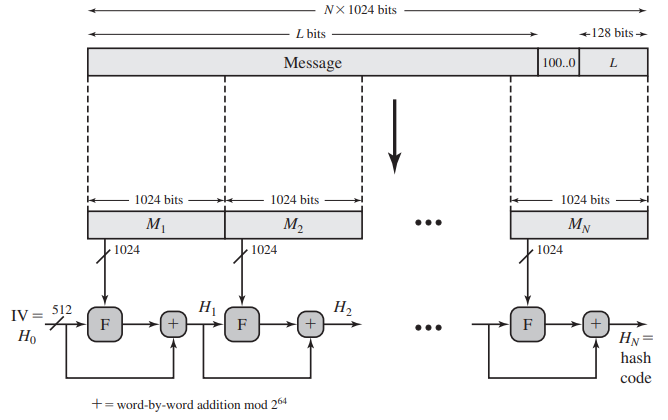
\includegraphics[width=\linewidth]{sha.png}
        \end{figure}

    \item \textbf{Output finale}
    
\end{enumerate}

\newpage

\begin{figure}[H]
    \centering
    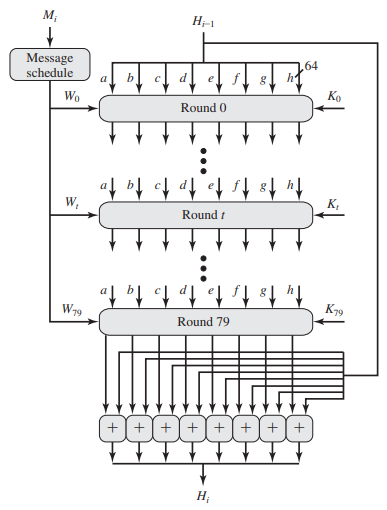
\includegraphics[width=0.7\linewidth]{sha2.png}
    \caption{Processo di un blocco nel dettaglio}
\end{figure}

\vspace{3pt}

\begin{itemize}
    \item $W_i$ deriva dal blocco corrente
    \item $K_i$ è una costante additiva
    \item Le operazioni svolte nel round sono quelle booleane primitive\newline
\end{itemize}

\subsubsection{Firma digitale}

La firma digitale consiste nell'aggiungere alla fine del messaggio l'output di una specifica funzione (DSA,ECDSA) che richiede la chiave privata del mittente e l'hash del messaggio stesso.\newline

\noindent Il destinatario potrà verificare che il messaggio è autentico facendo lo stesso procedimento con la chiave pubblica e confrontando l'output ottenuto con la firma presente.

\newpage

\subsubsection{HMAC}

Si tratta di un approccio basato su hash che serve ad autenticare i messaggi, permette di usare qualsiasi funzione di hash esistente senza modificare il procedimento.

\begin{figure}[ht]
    \centering
    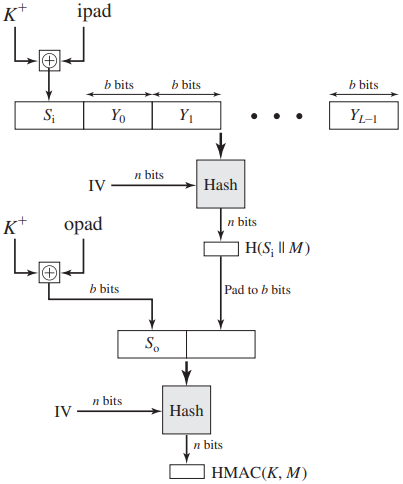
\includegraphics[width=0.7\linewidth]{hmac.png}
    \caption{Funzionamento}
\end{figure}

\begin{itemize}
    \item $H$ è la funzione di hash usata
    \item $M$ è il messaggio (compreso di padding se la funzione lo richiede)
    \item $Y_i$ è l'$i$-esimo blocco del messaggio
    \item $L$ è il numero di blocchi di $M$
    \item $b$ è il numero di bit per blocco
    \item $n$ è la lunghezza dell'hash prodotto
    \item $K^+$ è la chiave con eventuale padding di zeri a sx lunga $b$
    \item $ipad=00110110$ ripetuto $\frac{b}{8}$ volte
    \item $ipad=01011100$ ripetuto $\frac{b}{8}$ volte
\end{itemize}

\subsection{Altro}

\subsubsection{Certificazione della chiave pubblica}

Per garantire che una chiave pubblica sia effettivamente associata ad un individuo si usa un certificato composto da:
\begin{itemize}
    \item Chiave 
    \item ID del proprietario
    \item Firma di un terzo
    \item Altre informazioni
\end{itemize}

\noindent Il terzo è un'autorità certificata $CA$ che ha la fiducia della comunità.\newline

\begin{figure}[ht]
    \centering
    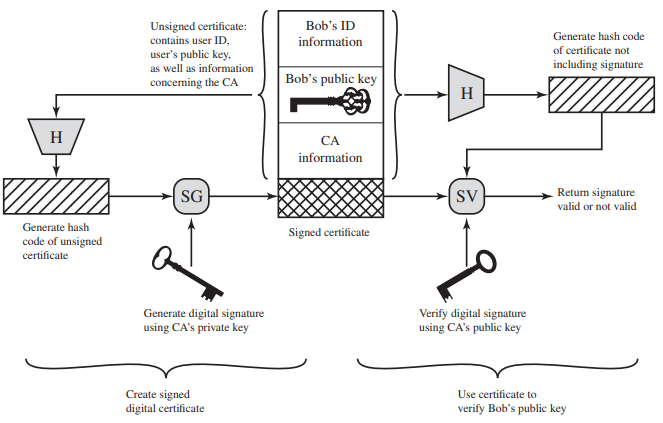
\includegraphics[width=\linewidth]{cert.png}
\end{figure}

\noindent Procedimento:
\begin{enumerate}
    \item Il client genera un certificato non firmato e lo invia in modo sicuro
    \item La $CA$ genera una firma digitale e la applica al certificato
    \item La $CA$ invia il certificato firmato al client
\end{enumerate}

\newpage

\subsubsection{Digital envelope}

Una tecnica che permette di inviare un messaggio cifrato combinando la cifratura asimmetrica con quella simmetrica usando una chiave simmetrica monouso:

\begin{figure}[ht]
    \centering
    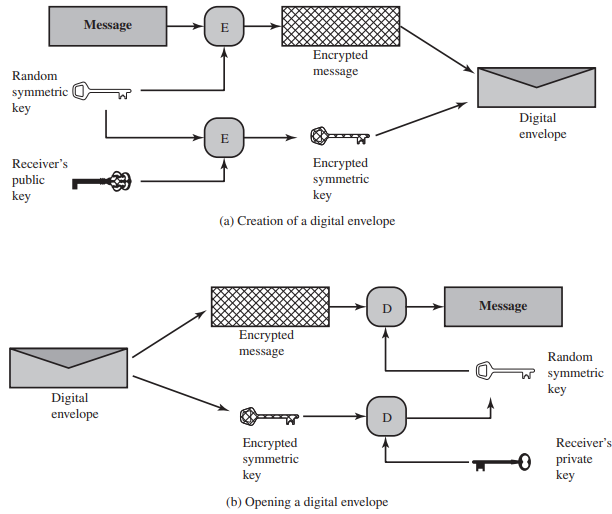
\includegraphics[width=0.8\linewidth]{de.png}
\end{figure}

\subsubsection{Cifratura dei dati memorizzati}

Alcuni casi di applicazione sono:
\begin{itemize}
    \item \textbf{Dispositivo HW backend}

        Viene posto tra i server e i sistemi di memorizzazione, cifra il traffico dai primi ai secondi e decifra quello opposto.
    
    \item \textbf{Cifratura basata su libreria}

        Si inserisce un coprocessore embedded con chiave integrata nei dispositivi appositi per i nastri magnetici.
    
    \item \textbf{PC}

        Esistono dei programmi che permettono di cifrare dischi o partizioni di essi.
    
\end{itemize}

\end{document}
